

\chapter{Metodologia}
W poniższym rozdziale opisano proces implementacji aplikacji mobilnej oraz modelu~rozpoznającego znaki języka migowego. 
Kluczowe elementy podczas tworzenia~oprogramowania obejmowały zarówno odpowiednie przygotowanie danych wraz z etykietami do późniejszej klasyfikacji, stworzenie aplikacji mobilnej jak i~integracja modelu z aplikacją.

Tworzenie kodu oparto na zasadach ,,czystego programowania'' (ang. Clean Code).
Takie podejście w programowaniu wymaga dbałości o czytelność, modułowość, łatwość rozbudowy oraz testowalność kodu.
Wszystkie komponenty kodu zostały zaprojektowane w sposób zapewniający jak największą przejrzystość oraz możliwość wielokrotnego wykorzystania.
Starano się implementować kod zgodnie z przyjętymi normami ,,czystej architektury'' (ang. clean architecture) w programowaniu w określonym frameworku.

\section{Implementacja modelu}
\subsection{Środowisko programistyczne}
Wybór środowiska programistycznego w celu implementacji modelu klasyfikującego znaki języka migowego podyktowany jest istniejącymi rozwiązaniami w dziedzinie wizji komputerowej. 
Ze względu na zastosowanie wytrenowanego modelu oraz ze względu na trywialność w przetwarzaniu danych wybór padł na język Python.

Dodatkową zaletą użytkowania ww. języka programowania wśród innych popularnych języków stosowanych w uczeniu maszynowym tj. R, Java czy C++, jest Anaconda.
Anaconda to darmowa, otwartoźródłowa dystrybucja języka Python (oraz R), zawiera ona wiele popularnych bibliotek używanych w uczeniu maszynowym, takich jak NumPy, pandas, scikit-learn, TensorFlow, Keras czy Jupyter Notebook.
Pozwala również na zarządzanie wirtualnymi środowiskami, a wraz z tym instalowaniem poszczególnych pakietów wymaganych do tworzenia oprogramowania.


Model na którym oparto prace pochodzi z badania proponującego przetwarzanie wideo jako sekwencji punktów orientacyjnych (ang. landmarks) dłoni, rąk oraz głowy wyekstraktowanych z poszczególnych klatek \footnote{Repozytorium kodu użytego w ww. badaniu dostępne pod \href{https://github.com/cristinalunaj/InterpretableTransformer_SignLanguage?tab=readme-ov-file}{tym linkiem}.} \cite{10.1145/3577190.3614143}.
Konkretnym zagadnieniem analizowanym w pracy jest stwierdzenie które punkty orientacyjne są znaczące w procesie klasyfikacji znaków języka migowego.
Oprogramowanie dostarczone przez autorów badania stanowi odpowiedni fundament w pracy nad aplikacją mobilną.

Jako model klasyfikujący użyto wyszkolonego modelu ,,SPOTERnoPE'' o dokładności $60.8\%$, który został wytrenowany na zbiorze stu klas pochodzących ze zbioru danych WLASL100 \footnote{Repozytorium kodu użytego do pozyskania zbioru danych dostępne pod \href{https://gist.github.com/wojteklu/73c6914cc446146b8b533c0988cf8d29}{tym linkiem}.}.

Wybór wyuczonego modelu podyktowany jest ograniczonymi zasobami obliczeniowymi, wymaganymi do wytrenowania modelu od podstaw.
Proces ten jest wymagający pod kątem nie tylko samej nauki ale i również wstępnego przetwarzania danych.
Dane które w kontekście tej pracy składają sie z filmów wymagają odpowiedniego przetworzenia na sekwencje klatek.
Dla dużych zbiorów danych które są wymagane w procesie uczenia modelu opartego na architekturze transformerów takie operacje wymagają nie tylko odpowiedniej architektury karty graficznej jak CUDA ale i również znaczącej ilości pamięci RAM.

Istotnym czynnikiem przemawiającym za wyborem wyżej opisanego modelu jest sposób klasyfikacji oparty nie na sekwencji klatek a na sekwencji punktów orientacyjnych.
Takie rozwiązanie pozwala modelowi skupić się w procesie uczenia jedynie na punktach orientacyjnych oraz zależnościami między nimi.
Tym samym niwelowane są aspekty takie jak m.in. tło czy jakość obrazu, które występowałyby w momencie uczenia na surowych obrazach, a które mogłyby przyczynić się negatywnie do znajdowania relacji pomiędzy sekwencjami klatek w procesie uczenia.


\subsection{Przygotowanie danych}
Zaimplementowany model przetwarza dane wejściowe w postaci tensora składającego się z sekwencji punktów orientacyjnych wyekstraktowanych z klatek filmów wideo.
Istotne jest zatem aby dane które mają zostać poddane klasyfikacji przechodziły przez ten sam proces wstępnego przetwarzania co dane użyte w procesie uczenia modelu.

Każdy film zatem dzielony jest odpowiednio na sekwencje klatek przy wykorzystaniu biblioteki OpenCV. Następnie klatki są przetwarzane tak aby uzyskać dane w postaci punktów orientacyjnych przy pomocy biblioteki MediaPipe.

\subsection{Analiza obrazów}
Analiza obrazów odbywa się na serwerze zewnętrznym opartym o framework Flask.
Zastosowanie architektury klient-serwer pozwala na utrzymanie modułowości oraz na skalowalność aplikacji.
Dodatkową zaletą zastosowania serwera Flask jest łatwe zarządzanie żądaniami HTTP.

Zastosowano stosunkowo prosty serwer zawierający jeden punkt końcowy (ang. endpoint) przyjmujący dane wideo zakodowane w formacie Base64.
Przesłane filmy są przetwarzane w celu wyekstraktowania punktów orientacyjnych, które następnie są przekazywane do modelu klasyfikującego. Wyniki klasyfikacji są zwracane do aplikacji mobilnej, gdzie są prezentowane użytkownikowi.

Warto jednak zaznaczyć, iż istnieją rozwiązania pozwalające na implementacje wytrenowanych modeli wewnątrz kodu źródłowego aplikacji mobilnej. 
Natomiast ze względu na złożoność zarówno implementacyjną jak i obliczeniową zdecydowano się na pominięcie takiego rozwiązania na rzecz architektury klient-serwer.


\section{Implementacja aplikacji mobilnej}
\subsection{Środowisko programistyczne}
Jako środowisko programistyczne do napisania aplikacji mobilnej wybrano Flutter. 
Flutter jest otwartoźródłowym zestawem do tworzenia oprogramowania stworzonym przez Google, który umożliwia tworzenie aplikacji wieloplatformowych z jednej bazy kodu źródłowego w tym aplikacji mobilnych na platformy Android i iOS.

W odróżnieniu od innych frameworków UI, które polegają na platformie docelowej w celu zapewnienia silnika renderującego, Flutter dostarcza aplikacje z własnym silnikiem renderującym ,,Skia'', co pozwala na identyczny wygląd aplikacji na wszystkich platformach docelowych.
Silnik ten komunikuje się z natywnymi zestawami SDK (ang. Software Development Kit), co pozwala na dostęp do funkcji specyficznych dla platformy, a w rezultacie pozwala zbudować aplikacje, niezależnie od platformy docelowej.


Flutter oparty jest na języku programowania Dart, który jest językiem zorientowanym obiektowo, ze składnią podobną do języka C oraz posiada wbudowany Garbage Collector.
Kod napisany w języku Dart jest kompilowany do kodu maszynowego, JavaScriptu lub WebAssembly \cite{dart_language_important_concepts}. 
Dodatkową zaletą korzystania z języka Dart jest system zarządzania zależnościami, który pozwala na łatwe dodawanie bibliotek zewnętrznych do projektu.

\subsection{Clean Architecture}
Podczas pisania oprogramowania aplikacji mobilnej zastosowano zasady ,,czystej architektury'' (ang. clean architecture).

Czysta architektura to paradygmat projektowania oprogramowania wprowadzony przez Roberta C. Martina,zwanym w środowisku programistycznym jako ,,wujek Bob'', którego celem jest tworzenie łatwego w utrzymaniu i skalowalnego oprogramowania poprzez organizowanie bazy kodu w odrębne warstwy z wyraźnymi zależnościami i obowiązkami. Filozofia ta opiera się na kilku zasadach, w tym Separation of Concerns (SoC), Dependency Injection i Single Responsibility Principle.
Takie podejście pozwala na łatwe rozbudowywanie aplikacji oraz na testowanie poszczególnych komponentów niezależnie od siebie, ponieważ każdy komponent jest od siebie odizolowany \cite{cleanArchitecture}.
Jak pokazano na rysunku \ref{fig:clean_atchitecture}, architektura zakłada istnienie czterech niezależnych warstw:

\begin{figure}[H]
    \centering
    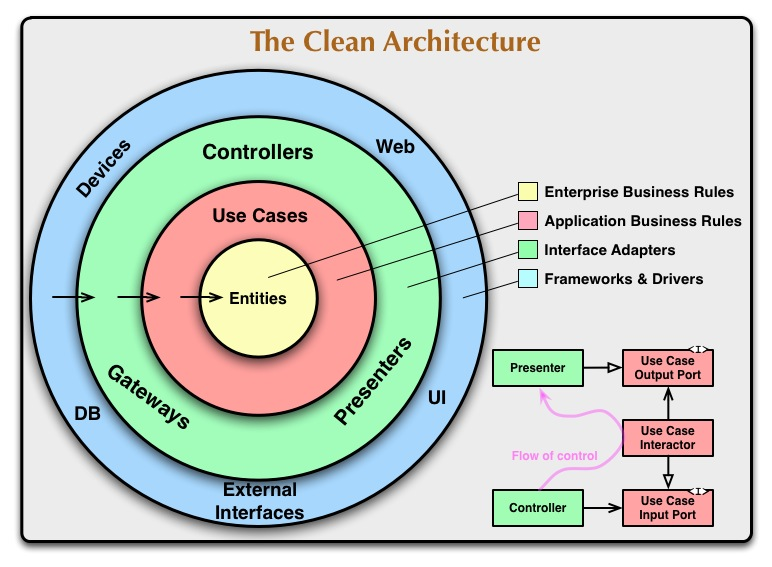
\includegraphics[width=0.75\linewidth]{figs/clean_architecture.png}
    \caption{Diagram przedstawiający strukturę ,,czystej architektury''.}
    \label{fig:clean_atchitecture}
\end{figure}

\begin{enumerate}
    \item Entities (Enterprise Business Rules) - jest najbardziej wewnętrzną wartswą. Zawiera obiekty, które reprezentują encje biznesowe, takie jak dane, logika biznesowa, reguły walidacji, itp.
    \item Use Cases (Application Buisness Rules) - warstwa ta definuje tzw. przypadki użycia, czyli akcje które użytkownicy mogą wykonać w aplikacji. Logika tej warstwy wywołuje odpowiednie metody z warstwy Entities. Jest ona niezależna od interfejsu użytkownika, bazy danych ani innych zewnętrznych szczegołów.
    \item Interface Adapters - warstwa odpowiedzialna jest za komunikacje pomiędzy warstwą przypadków użycia a zewnętrznymi interfejsami, takimi jak m.in. interfejs użytkownika.
    \item Frameworks and Drivers - jest to najbardziej zewnętrzna warstwa, zawiera szczegóły implementacyjne takie jak frameworki czy interfejsy użytkownika.
\end{enumerate}

Stosowanie ,,czystej architektury'' pozwala na łatwe wymienianie zależności w przypadku gdy którakolwiek z zewnętrznych części systemu stanie się przestarzała np. zmiana frameworka UI czy bazy danych.


\subsection{BLoC}
BLoC (Business Logic Component) pozwala na rozdzielenie warstwy prezentacji od logiki biznesowej.
BLoC może być efektywnie wykorzystany jako część ,,czystej architektury'', gdzie BLoC pełni rolę warstwy pośredniej między Use Cases a Frameworks and Drivers. 
Główną ideą BLoC jest zarządzanie stanem aplikacji poprzez przepływ danych oparty na zdarzeniach i reakcjach.

BLoC będąc pośrednikiem pomiędzy wymienionymi warstwami realizuje dwa kluczowe przepływy:
\begin{itemize}
    \item Zdarzenia (events): Warstwa użytkownika wysyła zdarzenia do BLoC, które reprezentują akcje wykonane przez użytkownika, np. kliknięcie przycisku czy wprowadzenie tekstu w polu formularza.
    \item Stany (states): W odpowiedzi na zdarzenia, BLoC generuje nowe stany, które są przesyłane z powrotem do warstwy prezentacji. Stany te opisują, jak interfejs użytkownika powinien się zmienić, aby odzwierciedlić aktualny stan aplikacji.
\end{itemize}
Przepływ danych przedstawiono na rysunku \ref{fig:bloc_diagram}.
\begin{figure}[H]
    \centering
    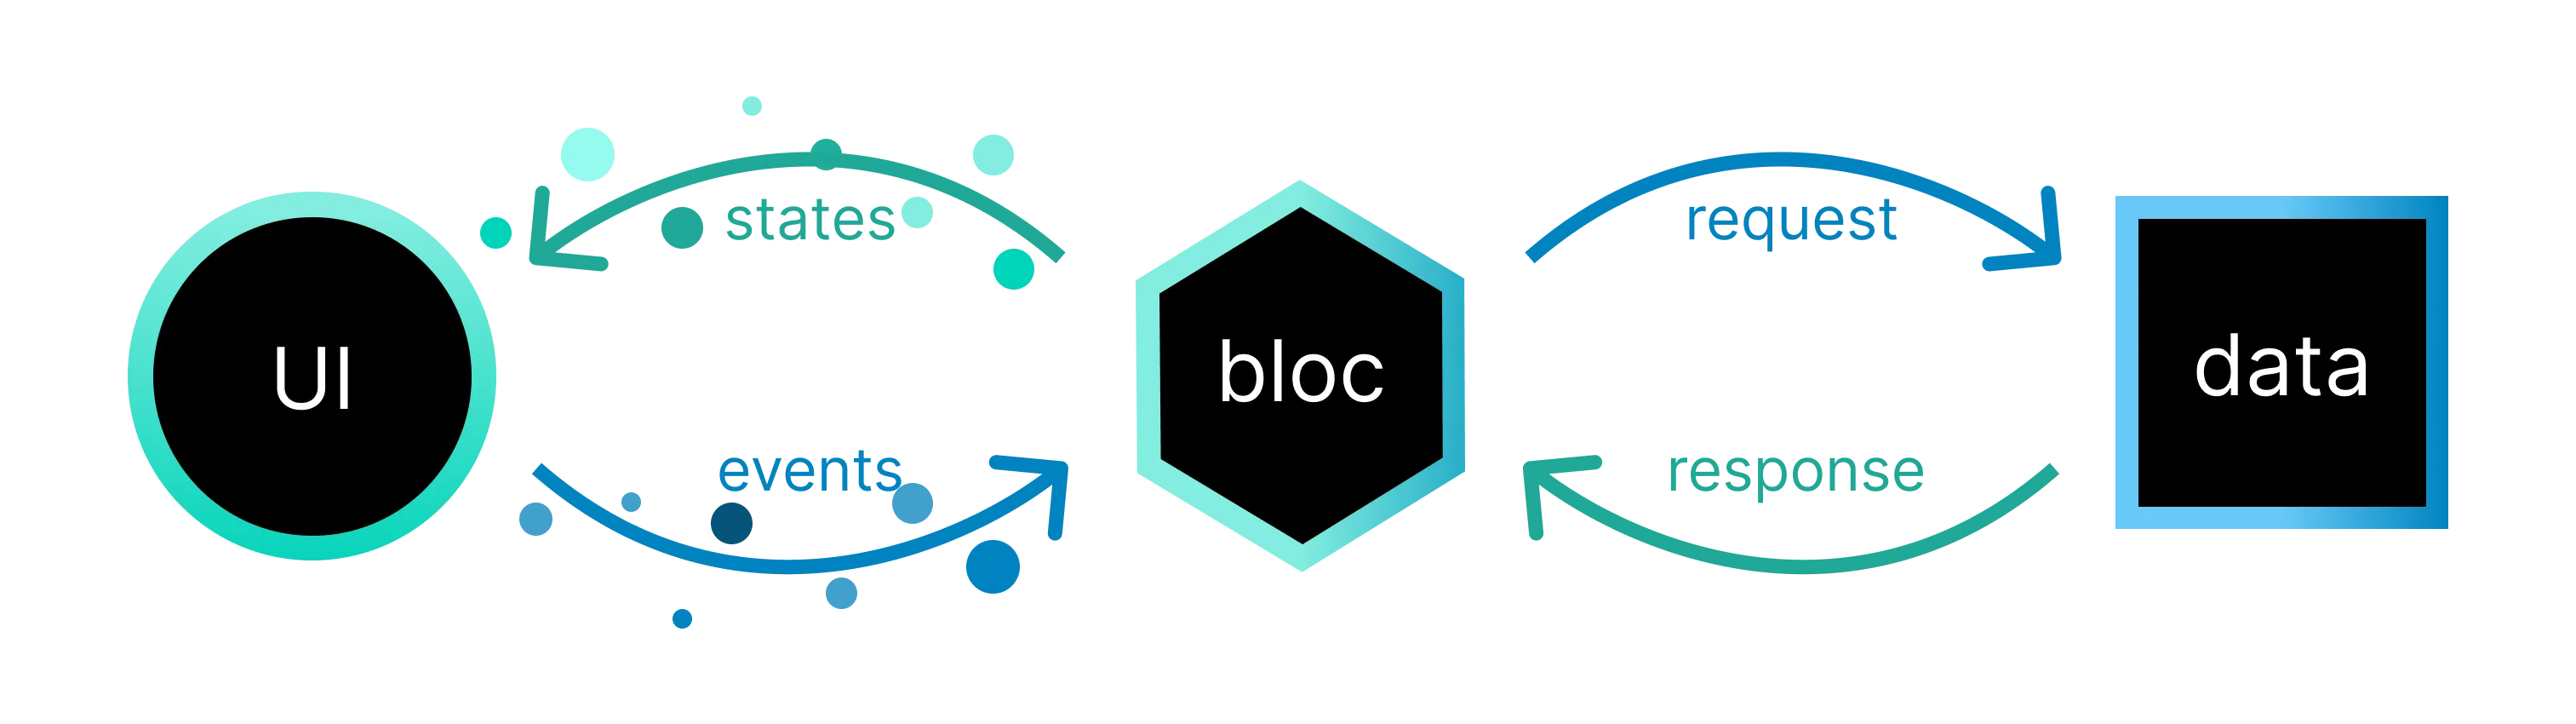
\includegraphics[width=0.9\linewidth]{figs/bloc.png}
    \caption{Schemat działania wzorca BLoC}
    \label{fig:bloc_diagram}
\end{figure}
Taki sposób ogranizacji kodu pozwala zachować jednokierunkowy przepływ danych, który minimalizuje błędy i ułatwia zarządzanie skomplikowanymi przepływami informacji w aplikacji.
%%%%%%%%%%%%%
% Na rysunku \ref{fig:bloc_diagram} przedstawiono przepływ danych w architekturze BLoC:
% - **UI:** Interfejs użytkownika, który generuje zdarzenia w odpowiedzi na interakcje użytkownika.
% - **BLoC:** Komponent pośredniczący, który odbiera zdarzenia, przetwarza je i generuje odpowiednie stany.
% - **Data:** Źródło danych, z którego BLoC pobiera informacje lub zapisuje zmiany w odpowiedzi na zdarzenia.

% Strzałki opisują przepływ informacji między poszczególnymi warstwami:
% 1. **Events (zdarzenia):** UI przesyła zdarzenia do BLoC.
% 2. **States (stany):** BLoC przetwarza zdarzenia i generuje nowe stany, które są przesyłane z powrotem do UI.
% 3. **Request i Response:** BLoC komunikuje się z warstwą danych, wysyłając żądania (request) i odbierając odpowiedzi (response).
%%%%%%%%%%%%%





\subsection{Struktura aplikacji mobilnej}

Biorąc pod uwagę powyższe założenia, struktura aplikacji mobilnej została zaprojektowana zgodnie z zasadami ,,czystej architektury'' oraz z wykorzystaniem BLoC jak pokazano na rysunku \ref{fig:app_structure}.

\begin{figure}[H]
\centering
\begin{forest}
    for tree={
      font=\ttfamily,
      grow'=0,
      child anchor=west,
      parent anchor=south,
      anchor=west,
      calign=first,
      inner xsep=7pt,
      edge path={
        \noexpand\path [draw, \forestoption{edge}]
        (!u.south west) +(7.5pt,0) |- (.child anchor) pic {folder} \forestoption{edge label};
      },
      before typesetting nodes={
        if n=1
          {insert before={[,phantom]}}
          {}
      },
      fit=band,
      before computing xy={l=15pt},
    }  
  [lib/
    [core/
    ]
    [shared/
    ]
    [features/
        [feature\_1/
            [data/
                [data\_sources/]
                [models/]
                [repository/]
            ]
            [domain/
                [repository/]
                [entities/]
                [use\_cases/]
            ]
            [presentation/
                [bloc/]
                [pages/]
                [widgets/]
            ]
        ]
        [feature\_n/
            [...]
        ]
    ]
    [l10n/
    ]
  ]
\end{forest}
\caption{Struktura katalogów aplikacji mobilnej}
\label{fig:app_structure}
\end{figure}

Przy tworzeniu odpowiedniej struktury kierowano sie zasadą ,,features first'', co oznacza, że kod powinien być zorganizowany wokół funkcjonalności, a nie typów plików.
Takie podejście pozwala na dodawanie nowych funkcjonalności do aplikacji bez konieczności zmiany istniejących plików. 
Dodatkowo tak struktura pozwala na ewentualne usunięcie danej funkcjonalności bez negatywnego wpływu na funcjonowanie kodu w pozostałej części aplikacji.

Istotnym problemem podczas implementacji ,,czystej architektury'' w aplikacji mobilnej o stosunkowo niedużej skali jest konieczność napisania kodu ,,boilerplate'', czyli kodu, który jest konieczny do napisania, ale nie wnosi wartości dodanej.
Sama struktura kodu początkowo staje się bardziej skomplikowana do implementacji, natomiast w dalszej perspektywie pozwala na zoorganizowane zarządzanie kodem aplikacji.